Nous allons consid\'erer les modifications de l'ensemble des ar\^etes de $G_{k,k'}$ afin d'obtenir un line-graphe. 
La premi\`ere modification  se base uniquement par ajout d'ar\^etes et la seconde sur la suppression d'ar\^etes uniquement. 
Nous supposons que les deux op\'erations conduisent sur la m\^eme borne sup\'erieure de $DL(G_{k,k'})$.

\subsubsubsection{Modification par {\em ajout d'ar\^etes uniquement}}
Soit le graphe $G_{k,k'}$ contenant $(k -1) \times (k'-1) + 1$ cellules.
Pour transformer chaque cellule en cliques comme cela est illustr\'e dans la figure \ref{exempleCorrectionGrapheCelluleAvecAjout}, nous ajoutons $2$ ar\^etes.
Nous consid\'erons le sommet $(0,0)$ contenu dans les cellules $C_{0,0}$ et $C_{k-1,k'-1}$.
Nous ajoutons $2$ ar\^etes dans $C_{0,0}$ et $C_{k-1,k'-1}$. Ces cellules deviennent des cliques $K_4$. 
\newline
L'ar\^ete $\{(i,j+1),(i+1,j)\}$ appartient aux cellules  $C_{i,j}$ et  $C_{i,j+1}$.
Or cette ar\^ete est d\'ej\`a couverte par une clique $K_4$ de la cellule $C_{i,j}$.
Alors nous ne pouvons pas ajouter d'ar\^etes dans la cellule $C_{i,j+1}$.
 L'ar\^ete $\{(i,j+1),(i,j+2)\}$ forme une clique $K_2$.
 Le sommet $(i,j+1)$ est couvert par une clique $K_4$ et une clique $K_2$. 
Le sommet $(i+1,j)$ est aussi couvert par une clique $K_4$ et une clique $K_2$ parce que les cellules $C_{i,j}$ et  $C_{i+1,j}$ partagent l'ar\^ete $\{(i+1,j),(i+1,j+1)\}$  et cette ar\^ete forme une clique $K_4$ avec la cellule $C_{i,j}$.
Les cellules $C_{i,j}$ et  $C_{i+1,j+1}$ ne partagent que le sommet  $(i+1,j+1)$. En plus les ar\^etes  $\{(i+1,j+1),(i+2,j+1)\}$ de  $C_{i+1,j}$ et  $\{(i+1,j+1),(i+1,j+2)\}$ de $C_{i,j+1}$ ne sont pas couvertes par une clique $K_4$. Nous pouvons alors transformer $C_{i+1,j+1}$ en une clique $K_4$  en ajoutant $2$ ar\^etes.
\newline
Ainsi, dans des cellules successives en lignes (avec $k$) ou en colonnes (avec $k'$), nous ajoutons des ar\^etes dans $\lceil \frac{k \times k'}{2} \rceil  + 1$ cellules. 
L'ar\^ete  d'une cellule qui n'est pas contenue par une clique $K_4$ forme une clique $K_2$.
Les cellules ayant un seul sommet en commun sont transform\'ees en des cliques $K_4$. 
\newline
\`A la fin  de la correction, la grille boucl\'ee $G_{k,k'}$ est partitionn\'ee en des cliques finies $K_4$ et $K_2$.
Dans cette construction, nous remarquons que chaque sommet est couvert par $2$ cliques. De cette construction d\'ecoule le lemme suivant :

\begin{lemma}
La distance line d'un graphe cellule $G_{k,k'}$ avec l'op\'eration  {\em ajout uniquement} est 
\begin{equation}
DL(G_{k,k'}) \le k \times k' +3 
\end{equation}
\end{lemma}

% ---- figure exemple correction graphe cellule G_{4,4}
\begin{figure}[htb!] 
\centering
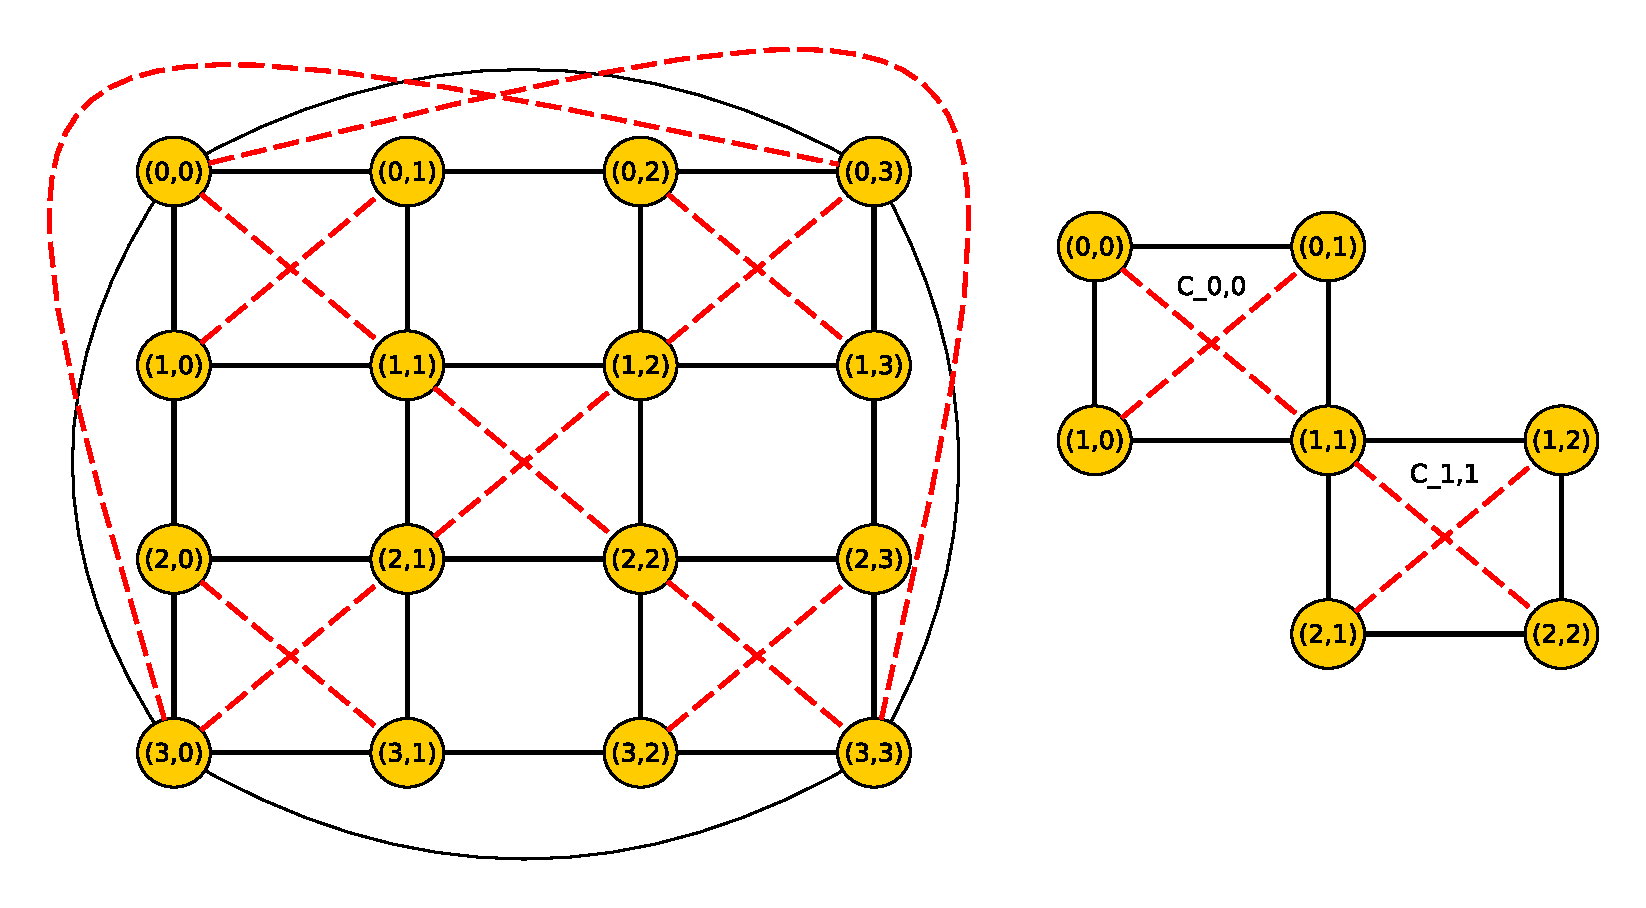
\includegraphics[scale= 0.6]{exempleGrapheCelluleAjoutG33.eps}
\caption{ La grille boucl\'ee  corrig\'e $G_{4,4}$ : elle est compos\'ee de $16$ sommets, $33$ ar\^etes. Il contient $4$ cliques $K_{2}$ et $6$ cliques $K_4$. Les ar\^etes ajout\'ees sont les traits de couleur rouge.}
\label{exempleCorrectionGrapheCelluleAvecAjout}
\end{figure}
% ---- figure exemple correction graphe cellule G_{4,4}
Dans la figure \ref{exempleCorrectionGrapheCelluleAvecAjout}, nous r\'ealisons la correction de distance line $DL(G_{4,4})  \le 12$ en transformant les cellules partageant un sommet en cliques $K_4$. C'est le cas des cellules $C_{1,2}$ et  $C_{0,2}$ qui ont le sommet $(1,2)$ en commun. 
Les ar\^etes partag\'ees entre deux cellules ont un des sommets couvert par une clique $K_2$ et l'autre sommet couvert par une clique $K_4$. Tel est le cas avec le sommet $(3,2)$ qui forme l'ar\^ete $\{(2,2),(3,2)\}$ et cette ar\^ete est contenue par une clique $K_4$.




\subsubsubsection{Modification par {\em suppression d'ar\^etes uniquement}}
\label{modificationSuppressionAretesUniquement}
Soit le graphe $G_{k,k'}$ contenant $(k-1) \times (k'-1) + 1$ cellules.
Nous supprimons les ar\^etes \\ $[\{(0,0),(k-1,0) \},  \{(0,0),(0, k'-1) \}, \{(k-1,0),(k-1,k'+1) \}]$ de la  cellule $C_{k-1,k'-1}$. Cette cellule contient uniquement  l'ar\^ete $\{(0,k'-1),(k-1,k'-1) \}$ et cette ar\^ete forme la clique $K_2$.
Nous supprimons \'egalement les ar\^etes $\{(0,k'-2),(0,k'-1)\}$ et $\{(k-2,k'-1),(k-1,k'-1) \}$  incidentes respectivement aux sommets $(0,k'-1)$ et $(k-1,k'-1)$ de sorte que ces sommets soient couverts par deux cliques $K_2$.
Les sommets de degr\'e minimums $(0,0)$, $(k-1,0)$. Ils sont couverts par deux cliques $K_2$ c'est-\`a-dire $\{(0,0),(1,0)\}$ et $\{(k-2,0) ,(k-1,0)\}$.
\newline
Consid\'erons les sommets de degr\'e $4$. Soit $(i,j)$ un tel sommet.
Pour former une bipartition autour de ce sommet, nous allons supprimer $2$ ar\^etes. Chaque ar\^ete appartient \`a deux cellules voisines. Dans notre cas, nous supprimons l'ar\^ete $\{(i-1, j), (i,j)\}$ entre les cellules $C_{i-1,j-1}$ et $C_{i-1,j}$ et aussi l'ar\^ete $\{(i,j), (i+1,j)\}$ entre les cellules $C_{i,j-1}$ et $C_{i,j}$. Ces sommets sont couverts aussi par des cliques $K_2$.
\newline
Les ar\^etes incidentes \`a un sommet de degr\'e $3$ et n'\'etant pas des cliques $K_2$ sont aussi supprim\'ees.
\newline
\`A la fin de l'algorithme de correction, la couverture de corr\'elation ne contient que des cliques $K_2$.
%Le graphe $G_{k,k'}$ est un cycle hamiltonien de  taille $(k \times k'+1) + k' + 1$.
Le graphe $G_{k,k'}$ est un graphe hamiltonien.
La distance de correction entre $G_{k,k'}$ et $L(G_{k,k'})$ est 
$DC_{k,k'} = (k-1) \times (k'-1) +3 $ 
et cette distance est minimale.

\begin{lemma}
La distance line  d'une grille boucl\'ee $G_{k,k'}$ avec l'op\'eration {\em suppression uniquement} d'ar\^etes est 
\begin{equation}
\label{borneSuperieureDL}
DL(G_{k,k'}) = (k-1) \times (k'-1) +3 
%DL_{supp}(G_{k,k'}) = k \times (k' +1) ===> cela correspond a quoi?
\end{equation}
\end{lemma}

% ---- figure exemple correction graphe cellule G_{3,3}
\begin{figure}[htb!] 
\centering
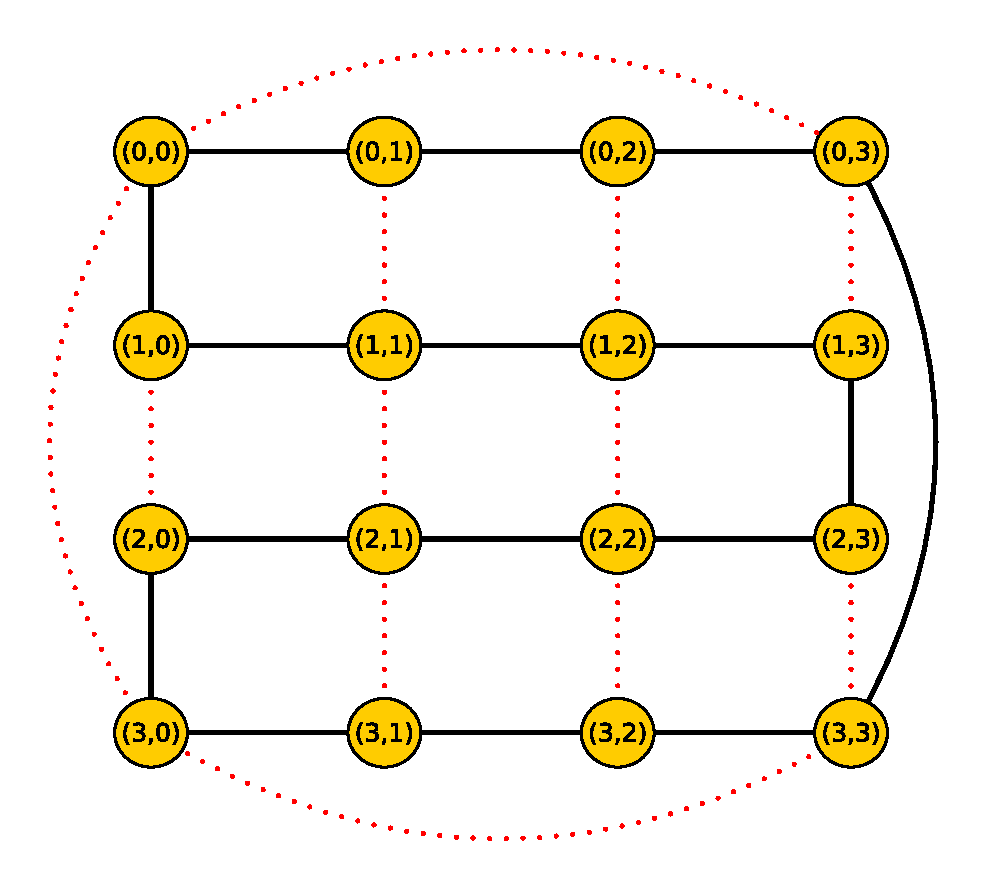
\includegraphics[scale = 0.7]{exempleGrapheCellulesSuppressionG33.eps}
\caption{ La grille boucl\'ee $G_{4,4}$ : elle est compos\'ee de $16$ sommets, $16$ ar\^etes et $16$ cliques $K_2$. Les ar\^etes supprim\'ees sont les traits en pointill\'ees rouges }
\label{exempleCorrectionGrapheCelluleAvecSuppression}
\end{figure}
%\FloatBarrier
% ---- figure exemple correction graphe cellule G_{3,3}
Une illustration de la correction avec l'op\'eration {\em suppression uniquement} est faite avec la grille $G_{4,4}$ dans la figure \ref{exempleCorrectionGrapheCelluleAvecSuppression}.
La grille $G_{4,4}$ poss\`ede $ k \times k' = 16$ cliques $K_2$ et $12$ ar\^etes sont supprim\'ees.
\newline

{\bf Conclusion} :
nous avons d\'etermin\'e deux types de modifications d'ar\^etes qui ont une borne sup\'erieure de la distance line pour chaque op\'eration. En revanche, les cliques formant la couverture de corr\'elation sont diff\'erentes selon la modification. Dans la modification {\em ajout d'ar\^etes uniquement}, le grille boucl\'e $G_{k,k'}$ contient des cliques $K_4$ et $K_2$ alors que  $G_{k,k'}$ ne contient que des cliques $K_2$ dans la {\em suppression d'ar\^etes uniquement}. 


